\documentclass{beamer}
\newcommand\Wider[2][3em]{%
\makebox[\linewidth][c]{%
  \begin{minipage}{\dimexpr\textwidth+#1\relax}
  \raggedright#2
  \end{minipage}%
  }%
}
\usepackage{tikz}
\usetikzlibrary{shapes,positioning,arrows.meta,fit,backgrounds}
\usepackage{multicol}
\usepackage{amssymb}
\usepackage{booktabs}
\usepackage{graphicx}
\usepackage{multirow}
\usetheme{default}
\setbeamertemplate{navigation symbols}{}
 
% ---- colors for node status ----
\definecolor{colCurrent}{RGB}{245,166,35}   % orange = being processed now
\definecolor{colDone}{RGB}{200,200,200}     % gray   = already processed (offline phase only)
\definecolor{colPending}{RGB}{255,255,255}  % white  = not processed yet
\definecolor{colTrue}{RGB}{140,200,140}     % green  = resolved via table lookup
\definecolor{colFalse}{RGB}{225,120,120}    % red



\begin{document}

\title{Detecção de ASSR em EEG via Redes Ocultas de Markov}
\author{Victor Ragazzi\\[2em]
Tiago Zanotelli\\
}
\date{ELT 610 - 21 de Setembro de 2026}
\frame{\titlepage}

%% ===================================================================
%% S2 -- Outline
\frame
{\frametitle{\LARGE Resumo da apresentação}
\Large
\begin{itemize}
    \item 01. Objetivo e contexto
    \item 02. Estados e observações
    \item 03. Janelamento do sinal
    \item 04. Cálculo da evidência estatística -- \textcolor{red}{CSM}
    \item 05. Treinamento da \textcolor{blue}{HMM}
    \item 06. Inferência usando a \textcolor{blue}{HMM}
    \item 07. Critérios de detecção
    \item 08. Resumo
\end{itemize}
}

\frame
{\frametitle{\LARGE 1. Objetivos e contexto}
\Large

O problema, detectar resposta cerebral a um estímulo auditivo

\begin{itemize}
    \item EEG contínuo + estímulo auditivo periódico;
    \item O cérebro sincroniza com o estímulo?
    \item Abordagem proposta: medir sincronia de fase nas frequências de estímulo por \textcolor{red}{CSM} e incorporar sua evolução temporal em uma HMM
\end{itemize}

\note{
Aqui a gente só contextualiza o problema, sem entrar em detalhes de implementação ainda.

O ASSR (Auditory Steady-State Response) é uma resposta cerebral evocada por um estímulo auditivo que se repete periodicamente (por exemplo, um tom modulado em amplitude a 40 Hz). Se o cérebro está processando esse estímulo, uma parte da atividade elétrica registrada no EEG passa a oscilar sincronizada com a frequência de modulação do estímulo.

O problema que queremos resolver é: dado um trecho de EEG gravado durante a estimulação, como decidir, de forma objetiva e automática, se existe ou não essa resposta sincronizada?

A abordagem clássica mede o grau de sincronia de fase entre as épocas do sinal nas frequências de estímulo e compara esse valor a um limiar estatístico. A CSM será usada como evidência observada, mas a decisão considerará também a persistência temporal dessa evidência.

O método que vamos apresentar hoje usa essa mesma ideia de sincronia de fase como \emph{evidência} instante a instante, mas incorpora essa evidência dentro de uma máquina de estados ao longo do tempo, em vez de tomar uma decisão única sobre o sinal inteiro. Isso é o que veremos a partir do próximo slide.
}
}

%% ===================================================================
%% S4 -- 2. Estados e observações
\frame
{\frametitle{\LARGE 2. Estados e observações}
\Large

\begin{itemize}
    \item Ao longo do tempo, o sistema está em um de \textbf{2 estados}: \textit{repouso} ou \textit{resposta}
    \item A cada janela, chega uma \textbf{observação}: o nível de evidência estatística:
    
    \begin{itemize}
        \item Ausente, baixo, médio, forte e muito forte;
    \end{itemize}
    \item A quantidade de níveis é configurável; a HMM recebe apenas o símbolo ordinal, não o valor contínuo
\end{itemize}
}

\frame
{\frametitle{\LARGE Como funciona uma HMM: exemplo prático}
\footnotesize
 
\begin{center}
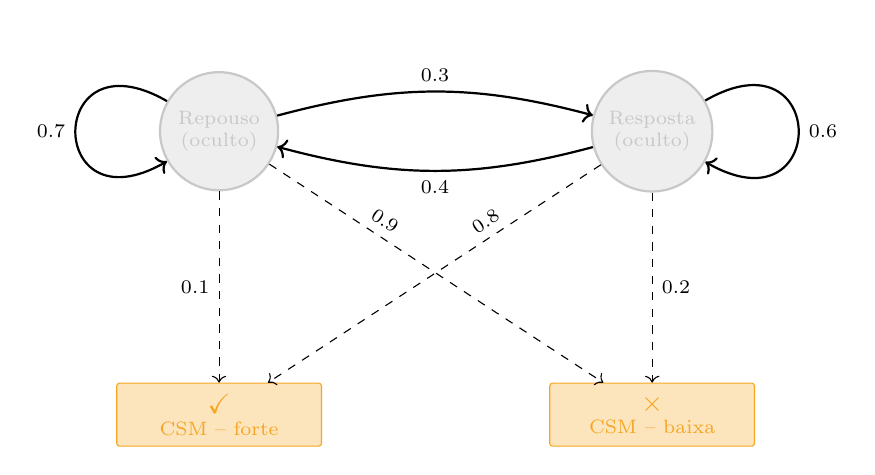
\begin{tikzpicture}[
    every node/.style={font=\scriptsize},
    state/.style={draw, circle, minimum size=1.5cm, align=center, thick},
    obs/.style={draw, rectangle, rounded corners=1pt, minimum height=0.8cm, minimum width=2.6cm, align=center}
]
    % hidden states (not observed directly)
    \node[state, colDone, fill=colDone!30] (E) at (0,3.6) {Repouso\\(oculto)};
    \node[state, colDone, fill=colDone!30] (C) at (5.5,3.6) {Resposta\\(oculto)};
 
    % self loops
    \draw[->,thick] (E) to[out=150,in=210,looseness=6] node[left]{0.7} (E);
    \draw[->,thick] (C) to[out=30,in=-30,looseness=6] node[right]{0.6} (C);
 
    % transitions
    \draw[->,thick] (E) to[bend left=15] node[above]{0.3} (C);
    \draw[->,thick] (C) to[bend left=15] node[below]{0.4} (E);
 
    % observations (what we actually measure), aligned under each state
    \node[obs, colCurrent, fill=colCurrent!30] (O1) at (0,0) {\normalsize$\checkmark$\\ CSM -- forte};
    \node[obs, colCurrent, fill=colCurrent!30] (O2) at (5.5,0) {\normalsize$\times$\\ CSM -- baixa};
 
    % emissions (dashed) -- straight edges = "own" observation, crossed = "other"
    \draw[->,dashed] (E) -- node[left,pos=0.5]{0.1} (O1);
    \draw[->,dashed] (C) -- node[right,pos=0.5]{0.2} (O2);
    \draw[->,dashed] (E) -- node[above,pos=0.32,sloped]{0.9} (O2);
    \draw[->,dashed] (C) -- node[above,pos=0.32,sloped]{0.8} (O1);
\end{tikzpicture}
\end{center}
 
\vspace{0.1cm}
Sequência observada: \ $\times \times \times \checkmark \checkmark$ \\
Estados ocultos inferidos: \textbf{Repouso, Repouso, Repouso, Repouso,} \textcolor{blue}{Resposta}
 
\note{
Esse slide mostra, com um exemplo concreto e bem conhecido da literatura, como uma HMM funciona de verdade -- antes de voltarmos para o nosso método no próximo slide.
 
A ideia clássica: imaginem que vocês estão trancados numa sala sem janelas, e querem saber se está chovendo lá fora. Vocês não conseguem observar o clima diretamente -- por isso ele é chamado de \emph{estado oculto}. O que vocês conseguem observar é uma pista indireta: se a pessoa que entra na sala está carregando um guarda-chuva ou não.
 
Nesse exemplo, temos 2 estados ocultos possíveis para o clima -- Ensolarado ou Chuvoso -- que mudam de um dia para o outro seguindo probabilidades fixas: por exemplo, se hoje está ensolarado, a chance de continuar ensolarado amanhã é 70\%, e a chance de virar chuvoso é 30\%; se hoje está chuvoso, a chance de continuar chuvoso é 60\%, e a chance de abrir o sol é 40\%. Essas são as chamadas probabilidades de \emph{transição} -- e a propriedade de Markov diz que essa probabilidade do dia seguinte só depende do estado de hoje, não do histórico inteiro antes disso.
 
O que vocês realmente enxergam -- a observação -- é se a pessoa trouxe guarda-chuva ou não, e essa observação também é probabilística: se está ensolarado, é raro (10\%) a pessoa levar guarda-chuva; se está chuvoso, é bem provável (80\%). Essas são as chamadas probabilidades de \emph{emissão}: a chance de cada observação, dado o estado oculto.
 
Juntando as duas coisas -- transição entre estados e emissão de observações -- dá para observar uma sequência de guarda-chuva/sem-guarda-chuva ao longo de vários dias, e usar um algoritmo (como o Viterbi, mencionado no slide anterior) para inferir qual é a sequência de estados ocultos (o clima) mais provável que gerou aquelas observações. No exemplo do slide, uma sequência de observações ``guarda-chuva, guarda-chuva, sem guarda-chuva, guarda-chuva'' tende a apontar para um clima majoritariamente chuvoso, com um dia de sol no meio.
 
Agora fazendo a ponte com o nosso problema: no lugar de ``Ensolarado/Chuvoso'', temos ``repouso/resposta''; no lugar de ``guarda-chuva/sem guarda-chuva'', temos o nível de evidência CSM discretizado. A matriz de emissão será calibrada uma vez a partir de ruído simulado e de uma heurística de inversão. Com essa matriz fixa, as probabilidades de transição serão estimadas a partir das sequências observadas.
}
}



%% ===================================================================
%% S5 -- 3. Janelamento do sinal
\frame
{\frametitle{\LARGE 3. Janelamento do sinal}
\Large

\begin{itemize}
    \item EEG contínuo dividido em \textbf{janelas deslizantes}
    \item Cada janela contém $N$ épocas do estímulo
    \item O passo entre janelas consecutivas é de $M$ épocas ($M \le N$)
    \item Resultado: uma \textbf{sequência ordenada} de janelas, cada uma gerando 1 observação
\end{itemize}

\begin{center}
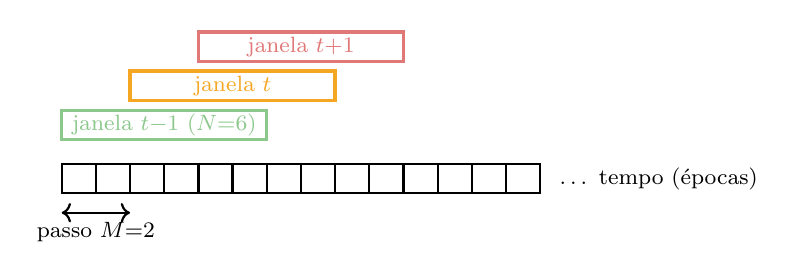
\begin{tikzpicture}[scale=0.62, every node/.style={font=\footnotesize}]
    % epoch timeline
    \foreach \i in {0,...,13} {
        \draw[thick] (\i*0.7,0) rectangle ++(0.7,0.6);
    }
    \node[anchor=west] at (14*0.7+0.2,0.3) {\ldots\ tempo (épocas)};

    % window 1 (N=6 epochs), step M=2
    \draw[thick, colTrue, line width=1.2pt] (0,1.1) rectangle ++(6*0.7,0.6);
    \node[colTrue] at (3*0.7,1.4) {janela $t{-}1$ ($N{=}6$)};

    \draw[thick, colCurrent, line width=1.2pt] (2*0.7,1.9) rectangle ++(6*0.7,0.6);
    \node[colCurrent] at (5*0.7,2.2) {janela $t$};


    \draw[thick, colFalse, line width=1.2pt] (4*0.7,2.7) rectangle ++(6*0.7,0.6);
    \node[colFalse] at (7*0.7,3.0) {janela $t{+}1$};

    \draw[<->, thick] (0,-0.4) -- (2*0.7,-0.4);
    \node[anchor=north] at (0.7,-0.4) {passo $M{=}2$};
\end{tikzpicture}
\end{center}
}

%% ===================================================================
%% S6 -- 4. Cálculo da evidência estatística (CSM) -- técnico
\frame
{\frametitle{\LARGE 4. Evidência estatística por janela -- CSM}
\Large

\begin{itemize}
    \item Para cada época $k$, extrai-se pela FFT a fase $\theta_k(f)$ nas frequências de interesse
    \item \textbf{Component Synchrony Measure}:
    $$\mathrm{CSM}(f) = \left|\frac{1}{K}\sum_{k=1}^{K}e^{j\theta_k(f)}\right|^2$$
    \item Calcula-se um \textbf{único valor por janela}, agregando frequências e canais
    \item A distribuição observada é dividida em $L$ categorias ordinais; $L$ acompanha automaticamente a lista de níveis definida no experimento
\end{itemize}
}

\frame
{\frametitle{\LARGE A CSM é intercambiável}
\Large

\begin{block}{Observação importante}
A \textcolor{red}{CSM} é a evidência escolhida aqui, mas \textbf{não é a única opção}: o restante do método não depende de como a evidência é calculada.
\end{block}

\vspace{0.3cm}
\begin{itemize}
    \item Pode-se trocar a CSM por \textbf{outro detector} (ex.: MSC, PLV ou teste $F$ espectral);
    \item Pode-se \textbf{fundir vários detectores} (usá-los como observações simultâneas/combinadas);
    \item Em ambos os casos, a estrutura da HMM (estados, matrizes probabilísticas e inferência) \textbf{não muda} -- só muda de onde vem a observação.
\end{itemize}

\note{
Vale reforçar esse ponto verbalmente na apresentação: a CSM entra no modelo apenas como fonte da \emph{observação} discretizada em cada janela. A HMM só enxerga níveis ordinais de evidência; de onde esses níveis vêm é intercambiável.

Isso mostra a modularidade da proposta: se a CSM se mostrar insuficiente, pode-se substituí-la por outro estimador ou fundir detectores antes da discretização, mantendo a mesma estrutura temporal.
}
}


%% ===================================================================
%% S7 -- 5. Treinamento da HMM
\frame
{\frametitle{\LARGE 5. Parametrização da HMM}
\large

\begin{itemize}
    \item Distribuição inicial fixa:
    $$\boldsymbol{\pi} = [P(\textit{repouso}),P(\textit{resposta})] \approx [0{,}95,0{,}05]$$
    \item Uma matriz de transição \textbf{compartilhada} entre condições:
    $$A_{ij}=P(S_t=j\mid S_{t-1}=i)$$
    \item Uma matriz de emissão \textbf{fixa e compartilhada}:
    $$B_{j\ell}=P(O_t=\ell\mid S_t=j)$$
    \item $B$ será calibrada uma vez com ruído e inversão normalizada; somente $A$ será ajustada aos dados reais
\end{itemize}
}

\frame
{\frametitle{\LARGE Calibração de $B$: repouso}
\large
\begin{itemize}
    \item Gerar blocos de ruído branco gaussiano, com a geometria de uma gravação de referência
    \item Aplicar o mesmo pré-processamento, janelamento e cálculo de CSM dos dados reais
    \item Discretizar usando os mesmos cortes por quantis definidos no conjunto de treinamento
    \item Contar as janelas em cada nível e adicionar pseudo-contagem $\alpha>0$:
    $$B_{\mathrm{rest},\ell} =
      \frac{n_\ell+\alpha}{\sum_{m=1}^{L}n_m+L\alpha}$$
    \item Registrar semente, número de simulações, amostragem, canais e parâmetros de janelamento
\end{itemize}
}

\frame
{\frametitle{\LARGE Calibração de $B$: resposta}
\large
\begin{itemize}
    \item Construir a linha de resposta por uma \textbf{heurística de inversão normalizada}:
    $$B_{\mathrm{response},\ell} =
      \frac{1/B_{\mathrm{rest},\ell}}
      {\sum_{m=1}^{L}1/B_{\mathrm{rest},m}}$$
    \item A pseudo-contagem garante que a inversão seja definida
    \item Níveis raros sob ruído recebem maior peso; isso pode incluir níveis baixos de CSM
    \item A regra não representa uma distribuição fisiológica de resposta estimada experimentalmente
    \item Um único $B$ será usado em 70, 50, 30 dB e ESP
\end{itemize}
\note{
A distribuição simulada usa ruído independente entre amostras e canais.
Ela é uma hipótese de referência, não uma reprodução completa do EEG em repouso.
Os cortes dependem dos dados de treinamento; portanto, a calibração não é
inteiramente independente dos dados reais. Trocar os cortes ou o processamento
exige recalibrar B. A inversão não garante crescimento monotônico com a CSM.
}
}

\frame
{\frametitle{\LARGE Treinamento não supervisionado de $A$}
\large
\begin{itemize}
    \item $\pi$ e $B$ permanecerão fixos durante todo o treinamento
    \item Forward--backward calcula as probabilidades das transições ocultas; o passo de reestimação atualiza \textbf{somente $A$}
    \item As transições esperadas serão somadas entre pacientes e condições, preservando as fronteiras de cada sequência
    \item Não serão necessários rótulos temporais nem máscaras de estímulo para inicializar $B$
    \item Pseudo-contagens regularizam $A$; múltiplos restarts perturbam apenas sua inicialização
    \item Será escolhida a solução de maior log-verossimilhança final
\end{itemize}
\note{
A inicialização de A favorece persistência nos estados. O protocolo não fixa
o instante de uma transição neural. As intensidades identificam sequências
independentes, mas não selecionam matrizes de emissão diferentes.
Com pseudo-contagens, o objetivo regularizado difere da verossimilhança pura;
esta última será usada para comparar os resultados finais dos restarts.
}
}


%% ===================================================================
%% S8 -- 6. Inferência usando a HMM
\frame
{\frametitle{\LARGE 6. Inferência: algoritmo de Viterbi}
\Large

\begin{itemize}
    \item Entrada: sequência de observações discretizadas, uma por janela
    \item Objetivo: encontrar a sequência de estados ocultos \textbf{mais provável} que explica essa sequência
    \item Viterbi = programação dinâmica que, a cada passo, combina:
    \begin{itemize}
        \item a probabilidade de emissão $B$ do nível CSM observado;
        \item a probabilidade de transição compartilhada em $A$;
    \end{itemize}
    \item Resultado: uma sequência repouso/resposta que considera a evidência e as probabilidades de transição
\end{itemize}
}

\frame
{\frametitle{\LARGE Ilustração: treliça de Viterbi}
\footnotesize

\begin{center}
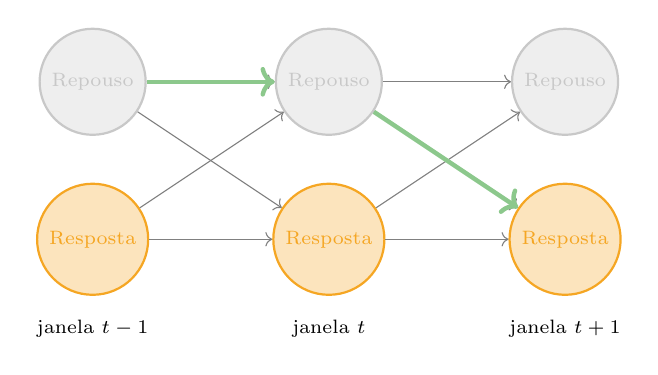
\begin{tikzpicture}[
    every node/.style={font=\scriptsize},
    st/.style={draw, circle, minimum size=1.0cm, align=center, thick}
]
    \foreach \t/\lab in {0/t-1, 1/t, 2/t+1} {
        \node[st, colDone, fill=colDone!30] (R\t) at (3*\t,2) {Repouso};
        \node[st, colCurrent, fill=colCurrent!30] (S\t) at (3*\t,0) {Resposta};
        \node[anchor=north] at (3*\t,-0.9) {janela $\lab$};
    }

    % all possible transitions (thin)
    \draw[->, thin, gray] (R0) -- (R1);
    \draw[->, thin, gray] (R0) -- (S1);
    \draw[->, thin, gray] (S0) -- (R1);
    \draw[->, thin, gray] (S0) -- (S1);
    \draw[->, thin, gray] (R1) -- (R2);
    \draw[->, thin, gray] (R1) -- (S2);
    \draw[->, thin, gray] (S1) -- (R2);
    \draw[->, thin, gray] (S1) -- (S2);

    % highlighted most-likely path
    \draw[->, thick, colTrue, line width=1.6pt] (R0) -- (R1);
    \draw[->, thick, colTrue, line width=1.6pt] (R1) -- (S2);
\end{tikzpicture}
\end{center}

\vspace{0.2cm}
\Large
Em \textcolor{colTrue!70!black}{\textbf{verde}}: caminho de maior verossimilhança encontrado pelo Viterbi (o que reportamos como estado inferido em cada janela)

\note{
Esse slide dá uma imagem mental de como o Viterbi escolhe o caminho entre todas as combinações possíveis de estados ao longo do tempo. A recursão combina $A_{ij}$ com a matriz de emissão compartilhada e fixa, $B_j(o_t)$. O treinamento e a inferência são etapas separadas: Baum--Welch estima somente $A$; Viterbi usa os parâmetros fixos para decodificar uma sequência.
}
}


%% ===================================================================
%% S9 -- 7. Critérios de detecção
\frame
{\frametitle{\LARGE 7. Critérios de detecção final}
\large

Depois de obter o caminho de estados inferido, ainda falta decidir: \textbf{houve ASSR ou não?}

\begin{itemize}
    \item Critério de persistência: exigir um número mínimo de detecções \textcolor{red}{consecutivas} e/ou uma proporção \textcolor{red}{mínima} de janelas em \textit{resposta}
    \item \textbf{Bandas de controle}: repetir todo o pipeline (janelamento + CSM + HMM) em frequências vizinhas, onde não há estímulo
    \begin{itemize}
        \item Representa uma condição onde não se espera resposta ao estímulo
        \item Usar os mesmos cortes, $B$ e $A$, sem novo ajuste; medir estados e sequências de resposta espúria
    \end{itemize}
    \item Comparação com o método clássico: esperamos taxa de falso positivo comparável, com potencial ganho de robustez temporal
\end{itemize}

\note{
Os limiares do critério final devem ser definidos antes da avaliação e tratados como hiperparâmetros. Exemplos são exigir pelo menos $X$ janelas consecutivas ou uma proporção mínima $Y$ de janelas no estado de resposta.

A ideia das bandas de controle é aplicar o mesmo processamento em frequências onde não se espera resposta neural. A taxa de estados ou sequências classificados como resposta funciona como diagnóstico de sobreajuste a ruído. Esse diagnóstico deve ser reportado, e não usado para corrigir silenciosamente o modelo.
}
}


%% ===================================================================
%% S12 -- 8. Resumo / fechamento
\frame
{\frametitle{\LARGE 8. Resumo: fluxo completo}
\footnotesize

\begin{center}
\resizebox{0.98\textwidth}{!}{%
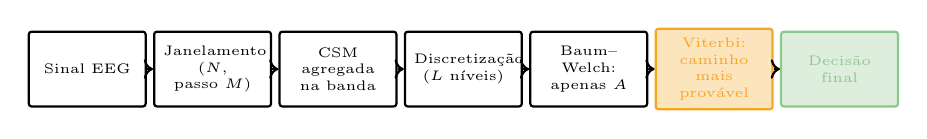
\begin{tikzpicture}[
    every node/.style={font=\tiny, align=center},
    box/.style={draw, thick, minimum width=1.45cm, minimum height=0.95cm, text width=1.25cm, rounded corners=1pt}
]
    \node[box] (sig) at (0,0) {Sinal EEG};
    \node[box, right=0.08cm of sig] (win) {Janelamento ($N$, passo $M$)};
    \node[box, right=0.08cm of win] (ev) {CSM agregada na banda};
    \node[box, right=0.08cm of ev] (disc) {Discretização ($L$ níveis)};
    \node[box, right=0.08cm of disc] (train) {Baum--Welch: apenas $A$};
    \node[box, right=0.08cm of train, colCurrent, fill=colCurrent!30] (tab) {Viterbi: caminho mais provável};
    \node[box, right=0.08cm of tab, colTrue, fill=colTrue!30] (dec) {Decisão final};

    \draw[->,thick] (sig) -- (win);
    \draw[->,thick] (win) -- (ev);
    \draw[->,thick] (ev) -- (disc);
    \draw[->,thick] (disc) -- (train);
    \draw[->,thick] (train) -- (tab);
    \draw[->,thick] (tab) -- (dec);
\end{tikzpicture}%
}
\end{center}

\vspace{0.4cm}
\Large
\begin{itemize}
    \item $\pi$ e $B$ fixos e compartilhados; somente $A$ estimada por \textbf{Baum--Welch}
    \item $B$: ruído gaussiano para repouso e inversão normalizada para resposta
    \item Caminho de estados calculado posteriormente via \textbf{Viterbi}
    \item Bandas de controle $\Rightarrow$ \textbf{taxa de falso positivo estimada} do método
    \item \textbf{Modularidade}: CSM pode ser trocada por outro detector, ou vários detectores podem ser fundidos, sem alterar a estrutura da HMM
\end{itemize}

}

\end{document}
